\documentclass[11pt,twocolumn]{report}
\usepackage{graphicx}
\usepackage{a4wide}
\usepackage[english]{babel}
\usepackage{amsfonts}
\usepackage{amsthm}
\usepackage{amsmath}
\usepackage{url}
\graphicspath{ {images/} }

\author{He Chen, Henri Maxime Demoulin, Gabrielle De Micheli}
\title{CIS520 Final Project Report}

\begin{document}
\maketitle
\section*{Introduction}
    In this report we detail our pre-processing steps, as well as four methods we analyzed during the project. We then proceed to an in depth analysis of the methods, and also present a visualization of the data which was instrumental in gaining accuracy.

\section*{Methods Accuracy Report}
    % Results for each method you tried (try to use checkpoints to get test set accuracy for each of your methods)
    First, let us explain the pre-processing steps that we have taken, in order to purify the features from low value words. We did delete all the English, French, and Spanish common stop words \cite{stopwords}, words containing only one character, Unicode words, words such as ``http'' and ``rt'', and a bunch of symbols not bearing emotions, such as ``--$>$'' or ``\_\_''. We tested multiple combinations of features removals, and observed that trimming too many "non emotional symbols", such as the ones we mentioned before, was not beneficial in terms of cross-validation error, nor in testing error on the leaderboard. We suppose that this is due to the correlation between such symbols and the other words in the text.
    \par
	Another thing that we have done, in order to check for words worth deletion, was to iterate through all $10,000$ of the word columns, and if deleting a column yielded significantly better cross validation accuracy ($1.5$ percent or better), then we deleted that column in the pre-processing step. However, the results where not as good as expected, and we ended up with a higher cross-validation error ($2$-$3$ percents) than we started with, so we did not include this part in our final preprocessing. 
    
    \subsection*{Generative Methods}
    \subsubsection{Naive Bayes}
    We start by using Naive Bayes only on the words. This method gave us around $80 \%$ testing accuracy on the leaderboard, without pre-processing. Adding a combination of the pre-processing described above, the testing accuracy raised to $81.42\%$. In order for Naive Bayes to work, we got rid of all the words that do not appear in any tweets, since it assumes conditional independence and $fitncb()$ does not handle words of probability $0$. We use a variation of the bag of words model, where the word counts is set to 1 if a word appears in a tweet and zero otherwise.
    \par
    We have also tried and tested $\log(w_i + 1)$ and $\sqrt(w)$, but doing that made the accuracy of Naive Bayes go bad $(22-35)$ percent of cross-validation error. So we concluded that the best way was simply checking if the word exists or doesn't exist (0 or 1). From our experience, Naive Bayes is both very accurate and extremely fast when used on the word counts.   
    \par
    We have also tried using the probabilities of each scene. For each example, we have set the highest probability image to 1, and set each other probability to 0, so it essentially becomes a One-Hot representation. Then, we removed each scene that did not appear in any of the examples, and ran multinomial Naive Bayes on it. We obtained 65 percent cross validation accuracy, which combined with the multinomial Naive Bayes on word counts resulted in 80 percent cross validation accuracy. We were not pleased with these results and therefore did not use this. 
   
    \subsection*{Discriminative Methods}

    \subsubsection{Linear Regression}
	We primarily did Linear Regression on the CNN features only. We tried it on the raw CNN features, the CNN features max pooled to various degrees, and the CNN features mean pooled to various degrees. At first we tried Elastic Net regression, which got around $65$ percent cross-validation accuracy, give or take $3$ percent for all of the different pooling methods. Then we tried $L1$ regression, which got pretty identical results as Elastic Net. Then we tried $L2$ regression which was slightly better than Elastic Net and $L1$, with about $68$ percent cross-validation accuracy.
    \par
    In all 3 of these regression methods, we were not able to get much better than $68$ percent cross-validation accuracy, which combined with the bag of words Naive Bayes, resulted in a $78-80$ percent cross-validation accuracy. Our conclusion was that linear regression was not appropriate for the CNN features, and so we did not incorporate it in our leaderboard model. 
    
     \subsubsection{Random Forest}
     We tried random forest on the words only and observed the following: with $20$ trees, cross-validation error was $0.2167$, while with $100$ trees it was $0.2116$. Cross-validation error stayed stable with $500$ and $1000$ trees, which is consistent with previous reports of random forest accuracy, where the model tends to overfit past the hundreds trees, without yielding much gain in accuracy \cite{latinne2001limiting,oshiro2012many}. We note that we used the same pre-processing steps we took with Naive Bayes.

    \subsubsection{SVM}
    Using SVM with an RBF (Radial Basis Function) kernel function, results in a cross-validation error of $0.3813$. With a linear kernel, the cross-validation error is $0.26$. However, we note that using RBF with the full word count (in lieu of the binary presence/absence indicator), we have a cross validation error of $0.3776$. Using the linear kernel with the full word count yields a cross-validation error of $0.2626$.
    
    \subsection*{Instance based Methods}
    \subsubsection{KNN}
    
    We use KNN on all four datasets and get a cross-validation error of 40 percent (give or take 5) with K clusters, K being 1 to 20. We decided not to use KNN not only due to the low individual accuracy, but also due to the low overall accuracy (78 to 80 percent) when combined with the other methods. We suspect that KNN is not very good for this kind of high dimensional classification because each point ended up being too far from the other points to make any good conclusions. 
   
    \subsection*{Semi-supervised methods}
    \subsubsection*{PCA}
    On the words, we tried PCA combined with SVM. With $570$ PCs, the threshold where the model grows past $50$MB, we got an accuracy of $0.7907$ on the leaderboard. Again on the words, and with that same number of PC ($570$), we used the PCA features with Random Forests and got a test accuracy of $0.7491$.

\section *{Methods Analysis}
    % Analysis of your experiments. What worked and what didn’t work? Why not? What did you do to try to fix it? Simply saying “I tried XX and it didn’t work” is not enough.

    Our first method, Naive Bayes, performed very well with the words, having extremely high velocity and also good accuracy. We think that this method fit very well with the data we have, partly because Naive Bayes performs better when examples are few, since it converges quickly. Also, we notice that Naive Bayes did not work very well with the images: this method is not supposed to work well with real values, and as we modified the structure of the features to force it to run (by setting the highest features to 1, and the other to 0, effectively discretizing the entire matrix), we were not surprised by the low accuracy.
    \par
    KNN performed globally very badly. The reason is very likely that our dataset is high dimensional, not really linearly separable, and KNN suffers from the curse of high dimensionality.
    \par
    We used Linear Regression various pre-processing of the CNN features, extensively experimenting max and mean pooling, as well as general feature scaling. We got poor results pretty much all the time, and got the suspicion that the set of images we were given are generally not helpful for telling appart joy and sadness. We concluded that Linear Regression was not appropriate for the CNN features, and did not incorporate it in our leaderboard model.
    \par
    Random Forest did perform quite well, one reason being that the structure of our data (many more features than observations) fits well with this method. Also, our understanding is that, as a mixture model, and as we have only two classes, the model is doing a very good job at capturing various flavor of joy and sadness. In the end, Random Forest did perform almost as good as Naive Bayes, but because it ended up being much more slower to compute and that the testing error was not quite as good as Naive Bayes, we chose the later.
    \par
    We tried SVM only on the words, and notice that it performed better than KNN but worse than Naive Bayes. The reason is that SVM exploits higher dimmensionality better than KNN, but can't beat Naive Bayes on the kind of data we are dealing with, because of the nature of Naive Bayes itself. We note that the RBF kernel performed much worse than the linear one, because it makes the model non parametric (while the linear kernel makes it parametric), which is totally against the mechanics of SVM (which is totally parameterized by the support vectors).
    \par
    Lastly, we observe that using Random Forest on PCA features was not significantly better than the native version, given the amount of PC we were able to use, but we suspect that our accuracy would have been much better with a higher number of PC, due to the fact that Random Forest is equally a good fit for the data (words) we have. We also notice that SVM on the PCA features performed worse than Random Forest on the same data, and suspect that it has to do with the poor linear separability of the words.
    \par
    Overall, Ensemble methods (RF) performed much better than non boosted ones, except for Naive Bayes, and the reason for that, we guess, is that Naive Bayes is simply very effective at this kind of categorical-bag-of-word classification with low number of examples (converges quickly). 

\section*{Visualization}
    % An interesting visualization of one of your models. For instance, find the words that most correlate with the outcome.
    In order to get a better sense of what words where most impactful during our classification, we consider the well-classified ones and use their count to create the word cloud bellow. Sadly, the engine we used got rid of some popular characters, such as ``\ldots'' and smileys.
    
    \begin{center}
        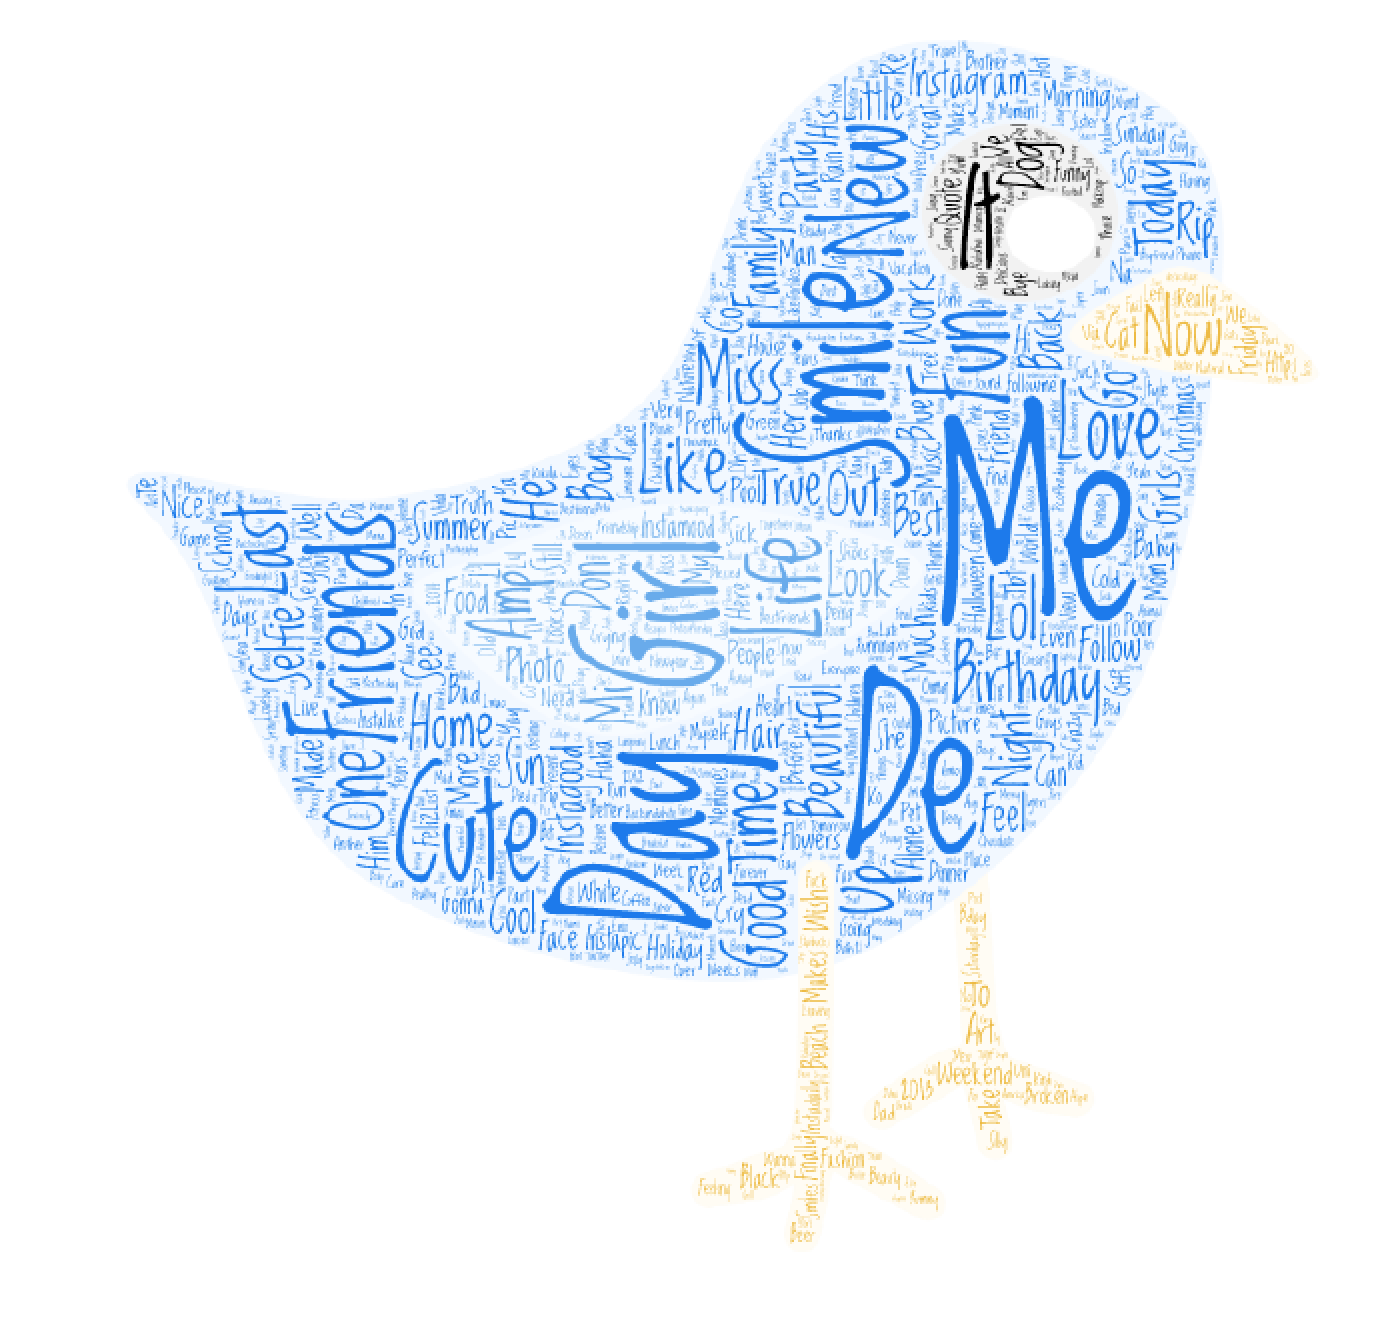
\includegraphics[scale=0.45]{cloud}
    \end{center}

\bibliographystyle{abbrv}
\bibliography{report}

\end{document}
